
%%%%%%%%%%%%%%%%%%%%%%%%%%%%%%%%%%%%%%%%%
% Journal Article
% LaTeX Template
% Version 1.4 (15/5/16)
%
% This template has been downloaded from:
% http://www.LaTeXTemplates.com
%
% Original author:
% Frits Wenneker (http://www.howtotex.com) with extensive modifications by
% Vel (vel@LaTeXTemplates.com)
%
% License:
% CC BY-NC-SA 3.0 (http://creativecommons.org/licenses/by-nc-sa/3.0/)
%
%%%%%%%%%%%%%%%%%%%%%%%%%%%%%%%%%%%%%%%%%

%----------------------------------------------------------------------------------------
%	PACKAGES AND OTHER DOCUMENT CONFIGURATIONS
%----------------------------------------------------------------------------------------
\documentclass[twoside,twocolumn]{article}

\usepackage[portuguese]{babel}
\usepackage{blindtext} % Package to generate dummy text throughout this template 
\usepackage[sc]{mathpazo} % Use the Palatino font
\usepackage[T1]{fontenc} % Use 8-bit encoding that has 256 glyphs
\linespread{1.05} % Line spacing - Palatino needs more space between lines
\usepackage{microtype} % Slightly tweak font spacing for aesthetics
\usepackage[utf8]{inputenc}
\usepackage{comment}

\usepackage[hmarginratio=1:1,top=32mm,columnsep=20pt]{geometry} % Document margins
\usepackage[hang, small,labelfont=bf,up,textfont=it,up]{caption} % Custom captions under/above floats in tables or figures
\usepackage{booktabs} % Horizontal rules in tables

\usepackage{lettrine} % The lettrine is the first enlarged letter at the beginning of the text

\usepackage{enumitem} % Customized lists
\setlist[itemize]{noitemsep} % Make itemize lists more compact

\usepackage{abstract} % Allows abstract customization
\renewcommand{\abstractnamefont}{\normalfont\bfseries} % Set the "Abstract" text to bold
\renewcommand{\abstracttextfont}{\normalfont\small\itshape} % Set the abstract itself to small italic text

\usepackage{titlesec} % Allows customization of titles
\renewcommand\thesection{\Roman{section}} % Roman numerals for the sections
\renewcommand\thesubsection{\roman{subsection}} % roman numerals for subsections
\titleformat{\section}[block]{\large\scshape\centering}{\thesection.}{1em}{} % Change the look of the section titles
\titleformat{\subsection}[block]{\large}{\thesubsection.}{1em}{} % Change the look of the section titles

\usepackage{fancyhdr} % Headers and footers
\pagestyle{fancy} % All pages have headers and footers
\fancyhead{} % Blank out the default header
\fancyfoot{} % Blank out the default footer
\fancyhead[C]{Breve História do Shell (e Unix)} % Custom header text
\fancyfoot[RO,LE]{\thepage} % Custom footer text

\usepackage{titling} % Customizing the title section

\usepackage{hyperref} % For hyperlinks in the PDF

\usepackage{graphicx}
\usepackage{float}

%----------------------------------------------------------------------------------------
%	TITLE SECTION
%----------------------------------------------------------------------------------------

\setlength{\droptitle}{-4\baselineskip} % Move the title up

\pretitle{\begin{center}\Huge\bfseries} % Article title formatting
\posttitle{\end{center}} % Article title closing formatting
\title{Breve História do Shell (e Unix)} % Article title
\author{%
\textsc{Guilherme Bittencourt Bueno da Silva} \\[1ex] % Your name
\normalsize Universidade Federal do Paraná \\ % Your institution
\normalsize {gbbs14@inf.ufpr.br} % Your email address
%\and % Uncomment if 2 authors are required, duplicate these 4 lines if more
%\textsc{Jane Smith}\thanks{Corresponding author} \\[1ex] % Second author's name
%\normalsize University of Utah \\ % Second author's institution
%\normalsize \href{mailto:jane@smith.com}{jane@smith.com} % Second author's email address
}
\date{\today} % Leave empty to omit a date
\renewcommand{\maketitlehookd}{%

%\begin{abstract}
%\noindent \blindtext % Dummy abstract text - replace \blindtext with your abstract text
%\end{abstract}
}

%----------------------------------------------------------------------------------------

\begin{document}

% Print the title
\maketitle

%----------------------------------------------------------------------------------------
%	ARTICLE CONTENTS
%----------------------------------------------------------------------------------------

\section{Introdução}

\lettrine[nindent=0em,lines=3]{C} om o avanço da tecnologia, a maneira de interagir com um computador mudou tanto que muitos usuários não precisam saber o que é um shell, a maioria dos usuários, nem precisam utilizar um shell.
Considerando que há 30 anos atrás, os usuários só tinham acesso ao mainframe através de uma estação com teclado e monitor para utilizar os comandos do shell, é possível dizer que hoje, computador é algo completamente diferente. Porém, hoje em dia, ainda usamos os mesmos termos para definir partes do sistema que hoje funcionam de maneira diferente. Então antes de apresentar a história do Shell, é bom diferenciar conceitos que são facilmente confundidos.

\section{Terminal vs Console vs Shell}

\subsection{Terminal}
Se você usa alguma distribuição unix, provavelmente já deve ter usado um terminal, mas certamente, não da mesma maneira que terminais eram utilizados antigamente. É fácil confundir e achar que o terminal está executando as operações, mas na verdade o terminal é apenas uma interface gráfica de um console. Pensando no terminal de antigamente é mais fácil entender que não é o terminal que executa os comandos: O terminal era algo físico, um ponto de acesso com meios de entrada e saída (teclado e monitor) para iteragir com a máquina, pois antes um computador era compartilhado por vários operadores.
Atualmente, cada usuário utiliza uma máquina diferente, e isso é um terminal:
\begin{figure}[h]
	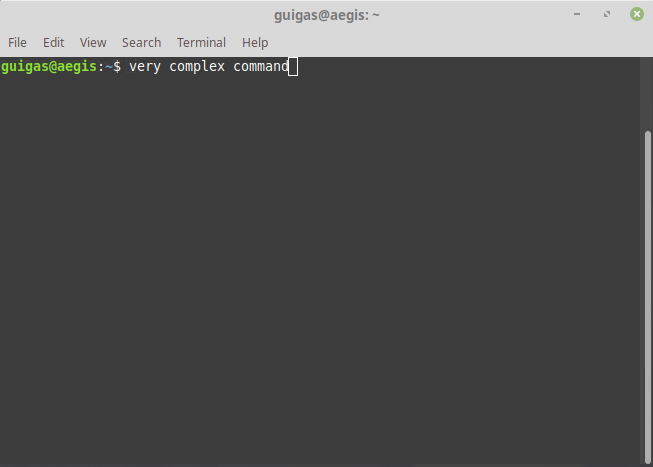
\includegraphics[width=\linewidth]{term2.png}
	\caption{Terminal atual.}
	\label{fig:term1}
\end{figure}
\subsection{Console}
Então, terminal é um meio de acesso a um console, mas os comandos que você insere também não são do console, e sim do Shell, mas voltando ao console, não é necessário um terminal para acessar um console. Em um sistema linux, apertando <ctrl> + <alt> + <F1 | F2 | ... | F6> é possível acessar um dos consoles (F7 para sair). Hoje, isso também é conhecido como o modo texto do seu sistema operacional, que é mais intuitivo que usar o termo console. Se um terminal era uma estação com tela e teclado, o console era a conexão física e digital entre o terminal e o mainframe. Então, Para cada sistema existe um console diferente, ligando cada sistema, a uma interface (geralmente, de texto), existem diferentes consoles para muitas coisas: BIOS, Boot Loader, init (processo incial do boot de sistemas unix). O console que está em uso quando você usa um terminal te da acesso ao Shell.
\subsection{Shell}
Shell possui esse nome pois ele funciona como uma casca separando o kernel do exterior. Sua função é servir de interface para acessar as funções do sistema operacional, tendo a vantagem de funcionar da mesma maneira em qualquer sistema operacional baseado em unix, escondendo detalhes específicos de cada SO.
\begin{figure}[h]
	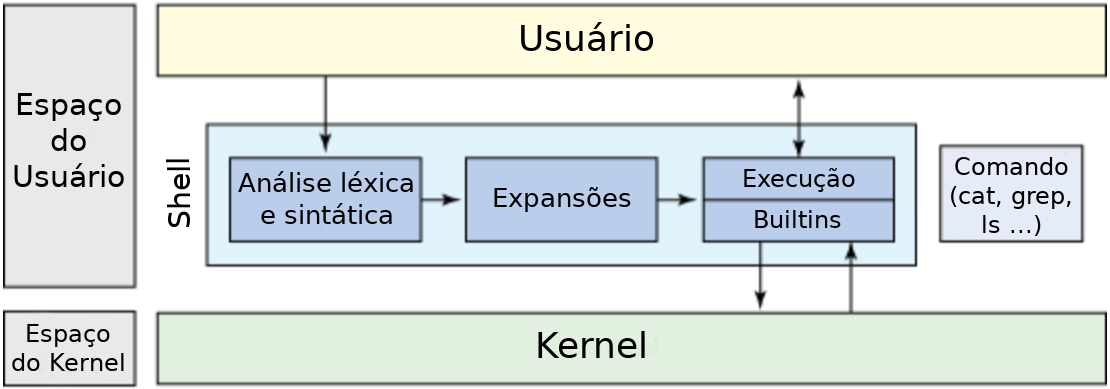
\includegraphics[width=\linewidth]{shell_struct1.png}
	\caption{Relação entre Shell, Kernel e usuário}
	\label{fig:shellstruct}
\end{figure}\\
Portanto, os comandos que você insere no terminal, são comandos do Shell que você está utilizando, que, na maioria dos sistemas linux atualmente, é o Bash. Diferentes Shells possuem funcionalidades diferentes, possivelmente implementadas com comandos diferentes, essas funcionalidades incluem:
\begin{itemize}
	\item Executar comandos.
	\item Manipulação de diretórios.
	\item Controle de processos (jobs).
	\item Expansões.
	\item Redirecionamento.
	\item pseudônimos (aliases).
	\item Histórico de comandos.
\end{itemize}
E muitas outras funcionalidades para facilitar, agilizar e automatizar as atividades realizadas.\\
Essas são algumas funcionalidades que estamos acostumados a utilizar hoje, mas nas primeiras versões de Shell, muitas delas não existiam.

\section{Unix, GNU, Linux e Shell}
Em 1971, Ken Thompson desenvolveu o primeiro UNIX Shell, chamado de V6 Shell (foi criado no Unix versão 6), e suas funcionalidades muito básicas, ele permitia pipes e redirecionamentos, mas ele estava mais próximo de um interpretador de comandos, ao invés de scripts\par
Dessa necessidade surgem novos Shells, com novas funcionalidades. Em 1977 foi criado o Bourne Shell, com dois objetivos: Servir como um interpretador de comandos e rodar scripts. Além disso, o Bourne Shell acrescentou ferramentas de controle (até então "if" existia como uma extensão, mas não era implementado diretamente no Shell V6), loops e variáveis, facilitando o uso de comandos e a criação de scripts. A partir disso surgem muitos outros Shells, e todos seguiram essas funcionalidades. Os principais foram: C-Shell, com o objetivo de deixar os scripts mais parecidos com a linguagem C. Korn Shell, que adicionou novas funcionalidades ao mesmo tempo que manteve forte compatibilidade com o Bourne Shell, e por fim, o Bourne Again Shell (Bash), que além de manter a compatibilidade com o Bourne Shell, também implementou as funcionalidades do C-Shell e Korn shell, ele também continuou a evoluir com o tempo, porém, um dos grandes facilitadores para o Bash ser o mais usado dos 3 é o fato de ele ser um projeto Open Source do GNU. \par
O projeto GNU não se trata apenas de criar uma versão open source do UNIX, mas sim de criar um ambiente onde sistemas abertos respeitam especificações e padrões, de modo que os usuários tivessem a liberdade para escolher, usar, distribuir e modificar software, e para isso é necessário que todo o sofwate: Sistema operacional, drivers, programas fossem software livre. Para isso a criação do Bash foi necessária, e com o sucesso do \href{https://www.gnu.org/gnu/manifesto.pt-br.html}{manifesto GNU}, o Bash foi o Shell mais difundido.
\section{Conclusão}
A maior evolução de qualquer Unix Shell foi a ideia de transformar o shell em uma ferramenta para Scripts, e não apenas um interpretador de comandos, essa mudança surgiu no Bourne Shell, e é bem provável que, qualquer que seja o Shell mais comum no futuro, continue sendo algum derivado do Bourne Shell, até que uma nova ideia que mude a maneira que usamos o Shell seja inventada.\par

%----------------------------------------------------------------------------------------
%	REFERENCE LIST
%----------------------------------------------------------------------------------------

\begin{thebibliography}{9} % Bibliography - this is intentionally simple in this template
	
	\bibitem[Evolution of Shells in Linux]{}
	\newblock https://www.ibm.com/developerworks/library/l-linux-shells/index.html
	\bibitem[What is the Difference Between Shell, Console, and terminal]{}
	\newblock https://fossbytes.com/difference-between-shell-console-terminal/
	\bibitem[O manifesto GNU]{}
	\newblock https://www.gnu.org/gnu/manifesto.pt-br.html
	\bibitem[A Brief History of Linux]{}
	\newblock https://www.digitalocean.com/community/tutorials/brief-history-of-linux
\end{thebibliography}

%----------------------------------------------------------------------------------------
\begin{comment}
\section{Methods}

Maecenas sed ultricies felis. Sed imperdiet dictum arcu a egestas. 
\begin{itemize}
\item Donec dolor arcu, rutrum id molestie in, viverra sed diam
\item Curabitur feugiat
\item turpis sed auctor facilisis
\item arcu eros accumsan lorem, at posuere mi diam sit amet tortor
\item Fusce fermentum, mi sit amet euismod rutrum
\item sem lorem molestie diam, iaculis aliquet sapien tortor non nisi
\item Pellentesque bibendum pretium aliquet
\end{itemize}
\blindtext % Dummy text

Text requiring further explanation\footnote{Example footnote}.

%------------------------------------------------

\section{Results}

\begin{table}
\caption{Example table}
\centering
\begin{tabular}{llr}
\toprule
\multicolumn{2}{c}{Name} \\
\cmidrule(r){1-2}
First name & Last Name & Grade \\
\midrule
John & Doe & $7.5$ \\
Richard & Miles & $2$ \\
\bottomrule
\end{tabular}
\end{table}

\blindtext % Dummy text

\begin{equation}
\label{eq:emc}
e = mc^2
\end{equation}

\blindtext % Dummy text

%------------------------------------------------

\section{Discussion}

\subsection{Subsection One}

A statement requiring citation \cite{Figueredo:2009dg}.
\blindtext % Dummy text

\subsection{Subsection Two}

\blindtext % Dummy text

%----------------------------------------------------------------------------------------
%	REFERENCE LIST
%----------------------------------------------------------------------------------------

\begin{thebibliography}{99} % Bibliography - this is intentionally simple in this template

\bibitem[Figueredo and Wolf, 2009]{Figueredo:2009dg}
Figueredo, A.~J. and Wolf, P. S.~A. (2009).
\newblock Assortative pairing and life history strategy - a cross-cultural
  study.
\newblock {\em Human Nature}, 20:317--330.
 
\end{thebibliography}

%----------------------------------------------------------------------------------------

\end{comment}
\end{document}
